\chapter{Test Bed and Design Decisions}
\label{chap:testbed}

%%%%%%%%%%%%%%%%%%%%%%%%%%%%%%%%%%%%%
%%%%%%%%%%%%%%%%%%%%%%%%%%%%%%%%%%%%%
%%%%%%%%%%%%   SECTION   %%%%%%%%%%%%
%%%%%%%%%%%%%%%%%%%%%%%%%%%%%%%%%%%%%
%%%%%%%%%%%%%%%%%%%%%%%%%%%%%%%%%%%%%
\section{Pros and Cons of the Existing Analysis}
\label{sec:mm:pros_n_cons}
The contribution of this thesis starts with scrutinizing the Existing Analysis. Upsides and downsides are investigated and verified to implement the best practice.
\subsection{Pros}
\label{mm:pros}
Existing analysis has considered every possible delicate detail to compute the worst case execution time. Upsides of the analysis are discussed here.

\subsubsection{Cache Miss}
Memory access time is different for different memory hierarchy levels. For instance, register memory can be accessed in one cycle, L1 cache in few cycles, L2 cache in 10 cycles and local DRAM needs approximately 100 cycles to be accessed by the CPU. To compute magnitude square root of 20 elements and store back the results to L1 cache, a core requires 280 cycles if the data are in L1 cache, 2140 cycles if the data are in SDRAM, assuming 4 cycles L1 access time and 10 cycle execution time per element. This kind of major variations are unfavourable for determinism. For safety critical systems the Worst Case Execution Time(WCET) needs to be analyzed and verified. The cache miss behaviour needs to be considered in the determination of the WCET. To achieve the worst case memory access times, it is assumed in the Existing Anlysis that a cache miss is produced for each memory access.

One of the ways to calculate Worst Case Execution Time (WCET) is to assume cache miss always. This is a pessimistic approach as the cache hit ratio is not always 0\%. 

\subsubsection{Memory Partitioning}
In time partition scheme, shared resources (L2 cache, Memory) are partitioned for A/A Mode and A/G mode to provide segregation. This isolation clearly defines the accessible address space for each core. Even if A/G mode processing of a core consumes huge memory space, A/A mode data of the core remains intact and will be useful during the next time slice. Another advantage of memory partitioning is load balancing. In Scheme-3 A/A mode analysis, 81\% of the core4's L2 partition is utilized whilst only 6\% of the core1's L2 partition is utilized. This quantitative information helps to reconfigure the partition values to have good load balance.

\subsubsection{CPU Utilization Balancing}
In time partition scheme, CPU utilization factors for A/A mode and A/G mode can be well balanced by configuring time slot period. For instance, in space partition scheme, core4 is utilized 75\% in A/A mode processing and 25\% in A/G mode processing. This information gives a hint for time partitioning that A/A mode needs more time span than A/G mode in core4. It is adopted in Scheme-2, allocating 14.5ms for A/A mode and 4.5ms for A/G Mode to balance the CPU utilization. Dynamic partition configuration can be considered in future to improve CPU load balancing.

\subsection{Cons}
\label{mm:cons}

\subsubsection{Context Switch Time}
Context switch time of 0.5ms is assumed for time partitioning. Every core does 2 context switches in 20ms. In time partition analysis (Scheme2 and Scheme3), at the end of 19.50ms all the four cores want to perform context switching. It is illustrated in Figure \ref{fig:mm:mm_cons1}. Since the SDRAM has only one port, it is possible for only one core to access the memory. Other cores have to wait till that time. 

\begin{figure}[h!]
	\centering
	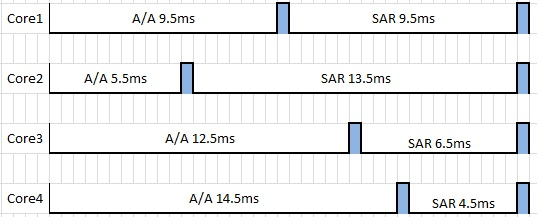
\includegraphics[width=120mm]{figures/mm_cons1}
	\caption{Time Partition of Scheme 3}
	\label{fig:mm:mm_cons1}
\end{figure}

Assuming the order of SDRAM access is core1, core2, core3 and core4. Core2 waits for core1 to complete (0.5ms), core3 waits for core1,2 (0.5ms + 0.5ms), core4 waits for core1,2,3 (0.5ms + 0.5ms + 0.5ms). This overhead in waiting time sums up to 3ms. Though only one context switch is contending, during the course of run it will be a scenario where two context switches will contend for SDRAM because of its skewed timing behaviour. Worstcase waiting time for four cores is 
\begin{align*}
	& = \frac{4*ContextSwitchTime \enspace + \enspace 2*OverheadInWaitingTime}{AvailableTime} \\[0.4cm]
	& = \frac{4*2*0.5ms \enspace + \enspace 2*3ms}{4*20ms} = 12.5\% \stepcounter{equation}\tag{\theequation} 
\end{align*}

In the worst case scenario, 12.5\% of the CPU time is spent only for context switching. This percentage is severe for a Radar processor. It degrades the application performance and much meaningful processing can be done during that time. \\

\textbf{\textsl{Verification:}} LMbench microbenchmark\cite{lmbench} is used to measure the context switch time of the ARM cores. LMbench is a free software suite of simple, portable benchmarks to compute various system performances including memory copy bandwidth, context switch latency, system call overhead, process creation latency, etc. Different sets of processes and data size are examined for the context switch time measurement. The LMbench suggests that the lowest recorded context switch time measurement is the more realistic one. So, lowest value of the 20 measurements are computed and listed in Table \ref{mm:ctxsw:lmbench}. 7.43$\mu$s in the table belongs to the context switch time measurement of two processes having 8KiB working data set each. The processes are scheduled according to the scheduling policy of the operating system. By monitoring the \verb|top| command, it is evident that the cores execute processes simultaneously, i.e. when four processes are involved in context switch, four cores are performing the execution.

\begin{table}[h!]
	\begin{tabularx}{\textwidth}{|X|X|X|X|X|}
		\hline
		\multirow{2}{*}{\textbf{Data Size [KiB]}} & \multicolumn{4}{c|}{\textbf{Context Switch Time[\boldmath$\mu$s]}} \\ \cline{2-5}
		& \textbf{2p} & \textbf{4p} & \textbf{8p} & \textbf{16p}  \\ \hline 
		8 & 7.43 & 9.09 & 12.76 & 13.58 \\ \hline
		16 & 8.22 & 16.35 & 19.31 & 20.87 \\ \hline
		32 & 9.57 & 18.48 & 23.68 & 29.13 \\ \hline
	\end{tabularx}
\caption{Measured Context Switch Time}
\label{mm:ctxsw:lmbench}
\end{table}

\begin{figure}[h!]
\centering
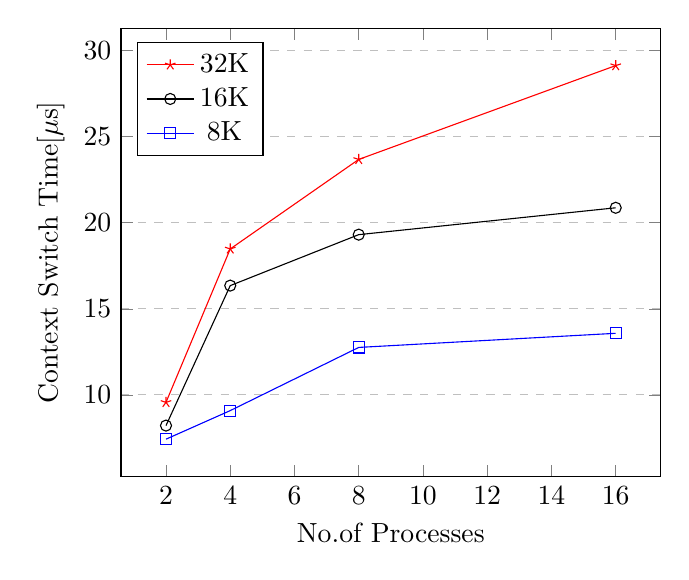
\begin{tikzpicture}
\begin{axis}[
	xlabel={No.of Processes},
	ylabel={Context Switch Time[$\mu$s]},
	legend pos=north west,
	ymajorgrids=true,
	grid style=dashed,
]
\addplot[color=red, mark=star,]
	coordinates {
		(2, 9.57) (4, 18.48) (8, 23.68) (16, 29.13)
	};

\addplot[color=black, mark=o,]
	coordinates {
		(2, 8.22) (4, 16.35) (8, 19.31) (16, 20.87)
	};
	
\addplot[color=blue, mark=square,]
	coordinates {
		(2, 7.43) (4, 9.09) (8, 12.76) (16, 13.58)
	};

	\legend{32K, 16K, 8K}
\end{axis}
\end{tikzpicture}
\caption{Comparison of Context Switch Time}
\label{mm:cntxt_switch_graph}
\end{figure}

From the above three sets of measurements, worst-case context switch time is 29.13$\mu$s corresponds to the 16 processes operating on 32KiB memory size. Also it reveals that the context switch time is proportional to the number of processes and data set size. On contrary to the assumption of 0.5ms context switch time and 12.5\% degradation in CPU utilization, measured worst-case context switch time is much lesser, therefore will not deteriorate the CPU utilization. So, no changes are made in the Existing Analysis with respect to the context switch time.

\subsubsection{Clashing Data Streams}
In time partition scheme, assume that the core1 of CPU1 is executing A/A Mode time slice. Now, A/G Mode data is routed to the same CPU by PSM2 as shown in Figure \ref{fig:mm:data_clash}. The core cannot accept the A/G Mode data as it is executing A/A time slice and the PSM have no idea of what the cores are up to or what to do with the data if the core is not accepting. This corner case is not clearly defined in the existing analysis, as a result it leads to data loss if no countermeasure is provided.

\begin{figure}[h!]
	\centering
	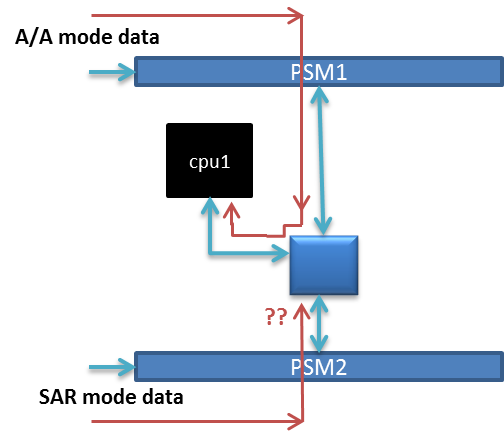
\includegraphics[width=80mm]{figures/data_clash}
	\caption{Clashing Data Streams}
	\label{fig:mm:data_clash}
\end{figure}

One of the ways to resolve this is to have a buffer in PSM to store the incoming data stream. If the core is not accepting the data, corresponding \verb|core_id| and \verb|cpu_id| shall be stored in the PSM along with the data. When the core is requesting data during next A/G Mode time slice, the PSM can transfer the stored data if the \verb|core_id| and \verb|cpu_id| matches. Since the incoming data stream is stored for one time slice period, it has to be counted for the processing latency calculation. The storing and restoring scheme ensures that the A/A data and A/G data will never be routed to the same CPU at the same time.

\subsubsection{Scalability}
\label{sss:mm:cons:scalability}
For time slot adjustment, it is cumbersome task to break the entire application into pieces such that each and every piece will fit in to one time slot. Whenever there is a change in time slot period, the entire application requires rework to suspend itself before the time slot expires. It implies that the time and cost of the application development and maintenance will increase. In addition, amendments are needed if the Radar configuration such as PRF set is changed.


\subsection{Other Comments}
\subsubsection{Typo}
Decimal conversion format(1000 Byte = 1KB) was used for byte conversion. This is changed to Binary conversion format (1024 Byte = 1KiB) to comply the standards. This has significant impact in the analysis results. An example is shown for interface utilization calculation of Scheme-1 in Chapter \ref{sec:scheme1:aa_interface_util}.

\begin{align*}
	\label{equ:mm:typo}
	iCON1 \: output \: to \: PSM1 &= \#\frac{byte}{sample} * \#channel * range \: gate * frequency \\
	&= 4 * 9 * 103 * 19.5kHz = 72306000 \frac{byte}{sec} = 72.3 \: MB/s \\
	Actual \: data \: rate &= \frac{72306000}{1024 * 1024} = 69 \: MiB/s \stepcounter{equation}\tag{\theequation}
\end{align*}

\subsubsection{Ideal Data Set Size}
Benchmarked functions have ideal data set range. For instance, matrix size of [1000 x 8] elements is processed to measure the execution time of complex multiply (CMY) function. Assuming 4 byte for a complex sample, 128-bit advanced SIMD unit (NEON) can hold four elements of CMYACC in a Q register and four multiplier elements in another Q register. Results of four multiplications are computed at the cost of one multiplication operation. But in reality, size of the data set is not always multiple of 128-bit. To compute CMY of [1000 x 9] data set, first eight elements of a row can be multiplied in SIMD lanes, last one element can be processed as normal multiplication operation. By doing so, it requires same execution time to process [1000 x 9] data set and [1000 x 12] data set, neglecting intrinsic load-store time. This performance constraint has to be taken into account for the full-fledged application development.

\subsubsection{OS Overhead}
Operating System overhead(OS Overhead) of 1.3 was included in the analysis. As the execution time are measured in \verb|Linaro| OS, redundant \textsl{OSoverhead} factor is removed for further analysis.

\subsubsection{Execution Cycle Mismatch}
\label{mm:cons:exe_cyl_mismatch}
Execution cycle reported in Chapter \ref{tbl:aa_exe} and the measured execution cycle of the benchmark functions do not match. The reported values are much lower than the actual measured values. These values are amended according to the measured values for Mode Mapping analysis. Table \ref{tbl:mm:aa_real_exe_cycle} shows the comparison of old values versus self measured values of the A/A Mode benchmarks.

\begin{table}[h!]
	\centering
	\begin{tabular}{|l|l|l|} 
	 \hline
	 \textbf{Benchmark} & \textbf{Old value [cycles]} & \textbf{Measured value [cycles]} \\
	 \hline
	 CMYACC8 & 79 & 287 \\ \hline
	 RMY50 & 15 & 68 \\ \hline
	 CONV128 & 24100 & 27300 \\ \hline
	 COT50 & 12 & 98 \\ \hline
	 FFT256 & 29700 & 37490 \\ \hline
	 MAG256 & 20 & 41 \\ \hline
	 AVG256 & 20 & 51 \\ \hline
	 CMPR256 & 7 & 55 \\ \hline
	 DET256 & 10 & 97 \\ \hline
	\end{tabular}
	\caption{Comparison of Old Execution Cycle vs Measured Execution Cycle of A/A Mode Benchmarks}
	\label{tbl:mm:aa_real_exe_cycle}
\end{table}

\FloatBarrier
\subsection{Measured Values of Existing Analysis}
\label{mm:cons:real_values}

The following processing latency and CPU utilization values are obtained for Existing Analysis, after updating the execution cycle values and removing OS overhead factor.

\subsubsection{Scheme-1}
\begin{table}[h!]
	\centering
	\begin{tabular}{|l|l|l|l|l|} 
	 \hline
	& \textbf{Core1} & \textbf{Core2} & \textbf{Core3} & \textbf{Core4} \\ \hline
	\textbf{Utilization} & 19.03\% & 46.20\% & 65.78\% & {\color{red} 108.07\%} \\ \hline
	\end{tabular}
	\caption{Measured CPU Utilization of Scheme-1, A/A Mode}
	\label{tbl:mm:scheme1_true_util}
\end{table}

\begin{table}[h!]
	\centering
	\begin{tabular}{|c|l|l|l|} 
	 \hline
	 \textbf{Look direction} & \textbf{Dwell time[ms]} & \textbf{Latency[ms]} & \textbf{\#Dwell latency} \\
	 \hline
	 1 & 27.84 & 416.40 & 14.96 \\ \hline
	 2 & 33.07 & 482.28 & 14.58 \\ \hline
	 3 & 39.17 & 574.52 & 14.67 \\ \hline
	 4 & 46.20 & 662.80 & 14.35 \\ \hline
	 5 & 54.26 & 798.62 & 14.72 \\ \hline
	\end{tabular}
	\caption{Measured Processing Latency of Scheme-1, A/A Mode}
	\label{tbl:mm:scheme1_true_latency}
\end{table}
\FloatBarrier

\subsubsection{Scheme-2}
\begin{table}[h!]
	\centering
	\begin{tabular}{|l|l|l|l|l|} 
	 \hline
	& \textbf{Core1} & \textbf{Core2} & \textbf{Core3} & \textbf{Core4} \\ \hline
	\textbf{Utilization} & 25.00\% & {\color{red} 103.33\%} & 71.43\% & 83.33\% \\ \hline
	\end{tabular}
	\caption{Measured CPU Utilization of Scheme-2, A/A Mode}
	\label{tbl:mm:scheme2_true_util}
\end{table}

\begin{table}[h!]
	\centering
	\begin{tabular}{|c|l|l|l|} 
	 \hline
	 \textbf{Look direction} & \textbf{Dwell time[ms]} & \textbf{Latency[ms]} & \textbf{\#Dwell latency} \\
	 \hline
	 1 & 27.84 & 860.00 & 30.89 \\ \hline
	 2 & 33.07 & 920.00 & 27.82 \\ \hline
	 3 & 39.17 & 1060.00 & 27.06 \\ \hline
	 4 & 46.20 & 1220.00 & 26.41 \\ \hline
	 5 & 54.26 & 1520.00 & 28.01 \\ \hline
	\end{tabular}
	\caption{Measured Processing Latency of Scheme-2, A/A Mode}
	\label{tbl:mm:scheme2_true_latency}
\end{table}
\FloatBarrier

\subsubsection{Inference}
The Existing Analysis will not meet real-time requirements as the CPU cores are utilized more than 100\%. Another down side is the 15x dwell latency, which is not in the acceptable range.

\clearpage
%%%%%%%%%%%%%%%%%%%%%%%%%%%%%%%%%%%%%
%%%%%%%%%%%%%%%%%%%%%%%%%%%%%%%%%%%%%
%%%%%%%%%%%%   SECTION   %%%%%%%%%%%%
%%%%%%%%%%%%%%%%%%%%%%%%%%%%%%%%%%%%%
%%%%%%%%%%%%%%%%%%%%%%%%%%%%%%%%%%%%%
\section{Test Procedure} 
\label{sec:mm:test_procedure}
Executable code is transferred to the Nitrogen6X board via Ethernet. Benchmark profiling are done as follows.

%%%%%%%%%%%%%%%%%%%%%%%%%
%%%%%   SUB-SECTION   %%%
%%%%%%%%%%%%%%%%%%%%%%%%%
\subsection{Memory Transfer Bandwidth}
\label{ss:mm:mem_bw}
STREAM benchmark\cite{McCalpin2007} is used to measure memory bandwidth of the machine. The STREAM benchmark is a simple, synthetic benchmark designed to measure sustainable memory bandwidth (in MB/s) and a corresponding computation rate for four simple vector kernels namely Copy, Scale, Add and Triad \cite{streamDef}. Peak achievable memory bandwidth is measured by running threaded STREAM benchmark on Nitrogen6X board. Only STREAM benchmark is started by the user to guarantee that the measurement is not affected by other user applications.  The STREAM benchmark is compiled and executed as follows: \\

\lstset{ %
  backgroundcolor=\color{mildyellow},
  numbers=left,
  numberstyle=\tiny\color{mygray},
  frame=single,
  showspaces=false,
  showstringspaces=false,
  basicstyle=\ttfamily,
}

\begin{lstlisting}
user$ gcc -fopenmp -D_OPENMP stream.c -o stream
user$ export OMP_NUM_THREADS=4
user$ ./stream
\end{lstlisting}

The measurement result of copying data from one memory location to another memory location is used for the  analysis. To measure the peak data transfer rate, the best result from 5 consecutive run is computed. As shown in Table \ref{tbl:mm:bw_no_load}, the iMX6Quad is capable of transferring \textbf{1048 MiB/s} when all the four cores are running in parallel.\\

\begin{table}[h!]
	\centering
	\begin{tabular}{|l|l|l|l|l|} 
	 \hline
	 \textbf{Function} & \textbf{Best Rate [MB/s]} & \textbf{Avg time[s]} & \textbf{Min time[s]} & \textbf{Max time[s]} \\
	 \hline
	 Copy & 1048.7 & 0.177625 & 0.152575 & 0.217059 \\ \hline
	\end{tabular}
	\caption{Idle Memory Transfer Bandwidth}
	\label{tbl:mm:bw_no_load}
\end{table}

To compute the peak memory bandwidth of the Radar application, STREAM benchmark is allowed to run in background along with the Radar application. STREAM is given low priority to give precedence to the Radar application. When the Radar application is consuming maximum bandwidth, STREAM can only consume the minimum leftover bandwidth. Subtracting minimum recorded bandwidth from the peak memory bandwidth of the iMX6Quad (1048 MiB/s), gives peak memory bandwidth utilized by the Radar application. Command for running STREAM benchmark at low priority: \\
\begin{lstlisting}
user$ sudo nice -n 19 ./stream >> ${OUTPUT_FILE}
\end{lstlisting}

%%%%%%%%%%%%%%%%%%%%%%%%%
%%%%%   SUB-SECTION   %%%
%%%%%%%%%%%%%%%%%%%%%%%%%
\subsection{Peak Memory Utilization}
\label{ss:mm:mem_util}
The percentage of the memory being used by a process can be extracted from \bverb|top| command. A bash script is written to read memory utilization 10 times a second (Appendix \ref{app:code:mem_util}) until the Radar application is running. The recorded peak memory utilization is exported to an output file for further analysis. This script is also run in background at low priority along with the Radar application as follows.\\
\begin{lstlisting}
user$ sudo nice -n 19 ./mem_util.sh &
\end{lstlisting}

%%%%%%%%%%%%%%%%%%%%%%%%%
%%%%%   SUB-SECTION   %%%
%%%%%%%%%%%%%%%%%%%%%%%%%
\subsection{Processing Latency (Worst Case Execution time)}
\label{ss:mm:latency}
Proper way of measuring the worst case execution time includes the following steps:
\begin{compactitem} 
	\item All the cores are set to begin the execution simultaneously to produce maximum communication bandwidth.
	\item Cache data are invalidated before and after the measurements to ensure that the data is always fetched from memory.
\end{compactitem} 

\noindent
The below mentioned methods are followed to improve the determinisism:
\begin{compactitem} 
	\item Every core executes a predefined thread.
	\item Radar application is given higher priority than other user space programs. \\
\end{compactitem} 

In worst case scenario, all the four cores will execute the same benchmark, generating maximum communication bandwidth, L2 cache contention and memory contention. To ensure that all the cores are executing the same benchmark, \bverb|wait_for_all_threads()| function is provided (Appendix \ref{app:code:wait_for_others}). A thread reaches this synchronization function waits utill all the other threads to join, afterwards all the threads begin benchmark execution simultanoously.

Invalidating cache data from user space is not allowed in ARM Cortex A9 processor. On the other hand, writing a program that copies huge junk of data from one memory location to other memory location seems to clear the cache contents. But, because of the complex caching strategies, it is not guaranteed that the entire cache data are removed, thus leaving major portion of the cache intact.\footnote{A discussion about this in ARM Connected Community forum can be found at \url{http://community.arm.com/thread/8799}} 

To overcome this, the Radar benchmark sequences are executed for 1000 iterations to measure the maximum execution time. A graph is drawn displaying the measured execution times during this 1000 iterations. However, there are some unexpected spikes ranging five times higher than the average execution time which occurs at sporadic intervals. The Nitrogen6X board is running \verb|ssh, GUI,| \\ \verb|network-manager|, background measurement tasks and other OS services along with the benchmark application. It can be reasoned that any of the other applications interrupts a running thread, causing it to be blocked for a while. So, the measurement is showing unrealistic values. The measured execution time of Comparison (\hyperlink{benchmarks}{CMPR256}) benchmark with spike and the resulting execution time after removing the spike are shown in Figure \ref{fig:mm:chop_off}.

\begin{figure}[h!]
	\centering
	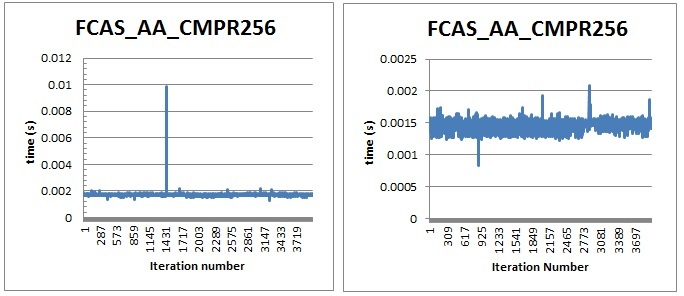
\includegraphics[width=150mm]{figures/chop_off}
	\caption{Before and After Spike Removal}
	\label{fig:mm:chop_off}
\end{figure}
A test run is made to study the effect of background tasks and services on the spikes. The background measurement tasks and services other than \verb|ssh, network-manager| are stopped. Now, only the minimal OS services are running. The Radar application is allowed to run in such less competitive environment. The result shows that the spikes are still occurring in few benchmarks, but the magnitude has reduced from 5x to 2x. As expected, some benchmarks do not have the spikes at all. It is concluded that the OS applications or services might have pre-empted the Radar application. Those spikes are removed from the graph and then the maximum execution time is computed. \vspace*{0.2cm}

To effectively utilize all the available four cores, four threads are spawned from main thread to carry out the parallel execution. Core affinity of each thread is set such a way that four threads are mapped to four cores (Appendix \ref{app:code:core_affinity}). For example, thread1 will run on core1, thread2 on core2, thread3 on core3 and thread4 on core4.\\
The Radar application is given higher priority than other user space tasks to give precedence. The following command is issued on Linaro Linux. 
\begin{lstlisting}
user$ sudo nice -n -20 ./AA_space_partition
\end{lstlisting}

%%%%%%%%%%%%%%%%%%%%%%%%%
%%%%%   SUB-SECTION   %%%
%%%%%%%%%%%%%%%%%%%%%%%%%
\subsection{CPU Load}
\label{ss:mm:cpu_load}
CPU Load is the ratio of busy time to the total time. Busy time is the execution time on a particular CPU and total time is the time delay between two consecutive inputs to the same CPU. The CPU load says the percentage of utilization as well as the remaining buffer time for future growth. 50\% spare time is a healthy value for CPU load. This spare time can be used for health monitoring that reports hardware and software failures. By doing so, faults can be isolated and stopped from propagating.

%%%%%%%%%%%%%%%%%%%%%%%%%
%%%%%   SUB-SECTION   %%%
%%%%%%%%%%%%%%%%%%%%%%%%%
\subsection{A/A Mode Sequence of Execution}
By matching the A/A Mode Processing Chain explained in Chapter \ref{sec:bg_related_work:proc_chain} and the list of benchmarks in Chapter \ref{sec:ch2:benchmark_results}, the following benchmarks are chosen to mimic the A/A mode Radar processing chain.

\begin{longtable}{|p{1.6cm}|p{1.9cm}|p{1.7cm}|p{1.9cm}|p{6cm}|} 
	 \hline
	\multicolumn{3}{|l|}{\textbf{Processing Chain}} & \textbf{Benchmark} & \textbf{Description} \\ \hline
	 \multirow{3}{*}{\parbox{1.7cm}{Time Domain Processing}} & \multirow{2}{*}{\parbox{1.5cm}{Beamform-ing}} & Beamform-ing & CMYACC & Sum, Azimuth and Elevation channel data are complex multiplied and the results are summed up \\ \cline{3-5}
	 & & Weight-ing & RMY & 4 channel data are multiplied with weighting vector. \\ \cline{2-5}
	& \multicolumn{2}{|l|}{Pulse compression} & CONV & Pulse compression in frequency domain. \\ \hline
	
	\multirow{3}{*}{\parbox{1.7cm}{Frequency Domain Processing}} & \multicolumn{2}{|l|}{Corner turning} & COT & 4 channel input data are corner turned. \\ \cline{2-5}
	& \multirow{2}{*}{\parbox{1.7cm}{Frequency Domain Transformation}} & Window-ing & RMY & 4 channel data are multiplied with windowing vector. \\ \cline{3-5}
	& & FFT & FFT & Transform time domain data to frequency domain. \\ \cline{2-5}
	& \multicolumn{2}{|l|}{Amplitude calculation} & MAG & Magnitude calculation of the Sum channel and Guard chanel data. \\ \hline
\end{longtable}
\clearpage
\begin{longtable}{|p{1.6cm}|p{1.9cm}|p{1.7cm}|p{1.9cm}|p{6cm}|} 
	 \hline
	\multicolumn{3}{|l|}{\textbf{Processing Chain}} & \textbf{Benchmark} & \textbf{Description} \\ \hline
	\multirow{3}{*}{\parbox{1.7cm}{Detection Processing}} & \multicolumn{2}{|l|}{Area average calculation} & AVG & Area average calculation of the  Sum channel and Guard chanel data. \\ \cline{2-5}
	& \multirow{2}{*}{\parbox{1.7cm}{Threshold-ing \& Detection}} & Comparison & CMPR & Compare magniture and Area average to produce pre-alarm matrix. \\ \cline{2-5}
	& & Detection & DET & Detects if the alarms entered through sidelobes by comparing Sum channel alarms against Guard channel alarms. \\ \hline
	\caption{A/A Mode - Benchmark Selection}
	\label{tbl:mm:aa_seq_exe}
\end{longtable}

The benchmarks shall be executed as shown in Figure \ref{fig:bg_related_work:aa_seq} to mimic the Radar processing chain. Functions of the Correlation processing are not included here.The burst, leading to the large data set (N$_{pri}$=205, N$_{rg}$=64) is processed as per the sequence diagram and the results are used for mode mapping analysis. In the following figure, \textsl{3x CMYACC} means, computing \hyperlink{benchmarks}{CMYACC} for three channels.

\begin{figure}[h!]
	\centering
	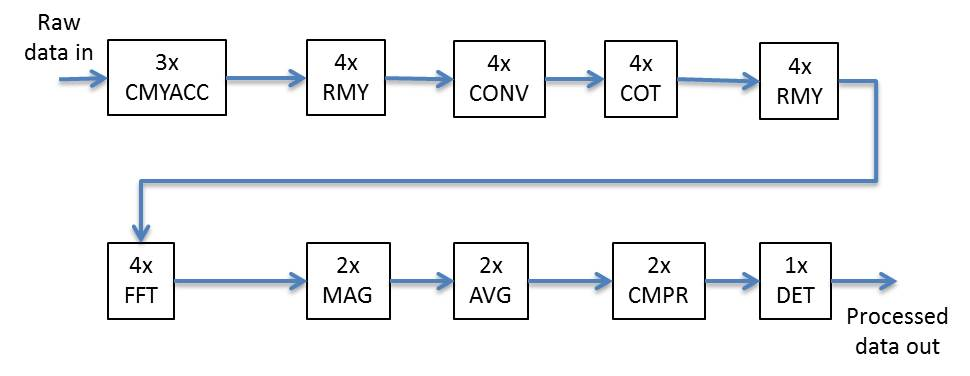
\includegraphics[width=160mm]{figures/aa_seq}
	\caption{A/A Mode, Sequence of Function Execution}
	\label{fig:bg_related_work:aa_seq}
\end{figure}

\clearpage
\section{Performance Comparison of Single Core vs Four Cores}
\label{sec:mm:perf_comp}
A performance comparison study has been done on the Nitrogen6X board equipped with ARM Cortex A9 quad core processor running the Radar benchmarks. In Figure \ref{fig:mm:1core_4core}, measurements of 1-thread, CMYACC means running CMYACC benchmark on core1 while other cores are idle. The figure implies that the four core performance is not as good as single core performance. Bottleneck is imposed by the shared resources L2 cache and Memory. In-case more than one core wants to access a shared resource simultaneously, only one core is allowed to access them at a given time. Other cores have to wait until the shared resource is freed again. This increases worst-case execution time of the benchmarks when running on four cores. The values used for the mode mapping analysis belong to the measurements of four core implementation.

\begin{figure}[h!]
	\centering
	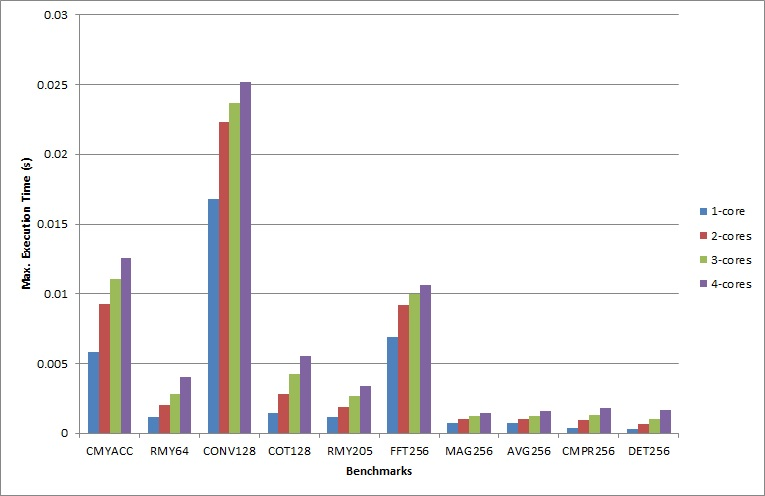
\includegraphics[width=140mm]{figures/1core_4core}
	\caption{Performance of Single Core vs Four Cores}
	\label{fig:mm:1core_4core}
\end{figure}


\clearpage
%%%%%%%%%%%%%%%%%%%%%%%%%%%%%%%%%%%%%
%%%%%%%%%%%%%%%%%%%%%%%%%%%%%%%%%%%%%
%%%%%%%%%%%%   SECTION   %%%%%%%%%%%%
%%%%%%%%%%%%%%%%%%%%%%%%%%%%%%%%%%%%%
%%%%%%%%%%%%%%%%%%%%%%%%%%%%%%%%%%%%%
\section{Design Decisions}
\label{mm:design_decisions}

\subsection{Parallel Execution}
Figure \ref{fig:mm:aa_serial_exe} illustrates the data distribution of Scheme-3 per CPU level. The diagram implies that the nature of execution is serial manner, in other words, it is equivalent to running the application on a single core processor. More CPUs and cores are used to improve the utilization factor, disregarding the processing latency. Thumb rule to reduce the processing latency is to process data independent portions of the application in parallel. 

\begin{figure}[h!]
	\centering
	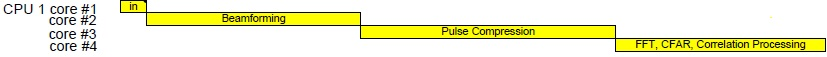
\includegraphics[width=160mm]{figures/aa_serial_exe}
	\caption{Serial Execution of A/A Mode Data in Existing Analysis}
	\label{fig:mm:aa_serial_exe}
\end{figure}

\subsection{Balanced Utilization}
In all the schemes of the Existing Analysis, core1 of the A/A Mode CPU does only Input/Output operations, utilizing a smaller amount of the available CPU capability. Due to this, other cores of the CPU have to carry out rest of the processing, leaving them over utilized. This kind of skewed utilization figure pushes up the CPUs worst case utilization factor, so having well balanced load is a gesture of a healthy system. Core1 should also take part in processing the Radar application for load balancing as well as latency reduction. \vspace*{0.2cm}

\subsection{Space Partition}
Evaluating the results of Time Partition scheme against Space Partition scheme, former one is considered to balance the CPU utilization by defining time slice periods. Down sides of the Time Partition scheme are:
\begin{compactitem} 
\item It magnifies latency by 2x compared to the Space Partition scheme.
\item As it requires breaking the entire application to fit into time slot, it is not scalable (see Chapter \ref{sss:mm:cons:scalability}).
\item Implementation needs more attention when it comes to memory partitioning.
\item Failure of one CPU will affect both the A/A mode and A/G mode processing.
\end{compactitem} 
\vspace*{0.2cm}
To sum up, Time Partition demands more effort and time to realise but producing no better result than Space Partitioning. So, this thesis decides to choose Space Partition as a base for further mode mapping analysis.

\subsection{Dedicated Communication Channels}
Distributing the Radar raw data to different CPUs and gathering processed data increases total amount of communication. As depicted in Figure \ref{fig:mm:dedicated_channels}, dedicated channels for input, output between the DGPM and PSM shall be established in Space Partition configuration. It facilitates receiving incoming data stream and sending out processed data simultaneously without interference. The DGPM has 6 port Ethernet interface, of which 4 port shall be connected to 4 CPUs and remaining 2 ports shall act as dedicated input, output channels.

\begin{figure}[h!]
	\centering
	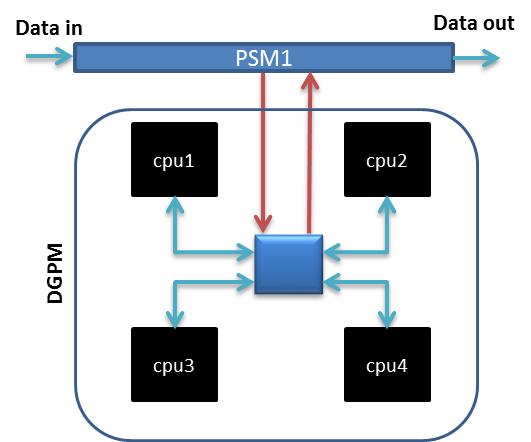
\includegraphics[width=60mm]{figures/dedicated_channels}
	\caption{Dedicated Communication Channels}
	\label{fig:mm:dedicated_channels}
\end{figure}

